\documentclass[11pt, titlepage]{article}
\usepackage[utf8]{inputenc}
\usepackage[czech]{babel}
\usepackage{a4wide}
\usepackage{graphicx}
\author{Martin Zadražil}
\title{Semestrální práce z~PC a PT}

\begin{document}

\begin{titlepage}
	\begin{center}
		
\includegraphics[width=10cm]{zculogo.ps}
		\vskip 5cm
		{\huge \bfseries Semestrální práce z~PC a PT} \\
		\vskip 1cm
		{ \large Martin Zadražil} \\
		{ \large \today }
	\end{center}
\end{titlepage}

\tableofcontents
\newpage

\section{Zadání}

Implementace jednoduchého šachového algoritmu, který umožňuje hru hráče proti počítači. Vstup a výstup bude probíhat na~příkazové řádce.

\section{Analýza úlohy}

Nejprve je potřeba navrhnout základní datové struktury a rutiny, které musí obsahovat každý šachový program i takový, který neobsahuje žádný myslící algoritmus a umožňuje například jen hru dvou lidských hráčů po síti. Patří sem funkce pro
\begin{itemize}
	\item nalezení všech legálních tahů z~dané pozice,
	\item kontrola šachu a matu,
	\item funkce kontrolující dodržení pravidel při~rošádě a braní mimochodem,
	\item funkce, která zahraje samotný tah.
\end{itemize}
Bude následovat umělá inteligence a chybět nesmí ani několik málo funkcí pro komunikaci s~okolím, jako je zparsování tahu zadaného z~klávesnice, vypsání tahu, upozornění na~přemýšlení programu a podobně.

\subsection{Umělá inteligence a teorie šachové hry}

\subsubsection{Od nejjednoduššího algoritmu ke kaskádové metodě}
Šachy jsou čistě matematickou úlohou, k jejímuž vyřešení se dá v~každém případě dopočítat. Za vyřešení úlohy můžeme považovat mat v~případě vyhrané pozice, pat v~případě remízové pozice nebo alespoň co největší oddalování porážky v~případě prohrané pozice. Klíčovou funkcí je statická ohodnocovací funkce, která vrátí číselnou hodnotu dané pozice. Nejjednodušší algoritmus, který nehraje úplně náhodně, vygeneruje všechny tahy ze zadané pozice, každý z~nich zahraje a vzniklou pozici ohodnotí statickou ohodnocovací funkcí. Pokud je hodnota pozice vyšší než dosud nejvyšší, uloží ji i tah, kterým jsme se na~ni dostali. Poté zahraje tah zpět a tak dále, dokud nevyzkoušíme všechny tahy. Tento algoritmus je sice lepší než náhodné generování tahů, ale přesto je velmi primitivní. Sebere klidně dámou krytého pěšce, nepokryje jednotahový mat a podobně.

Vylepšením je přidat rekurzi. Zahrajeme všechny tahy z~dané pozice, na~tyto tahy zahrajeme odpověď soupeře, pak zase naši odpověď a tak dále až do~nějaké hloubky~n, kde zavoláme statickou ohodnocovací funkci. Tento algoritmus se jmenuje minimax. Na šachovnici je v~základním postavení 16 pěšců, každý z~nich může táhnout nejvýše šestkrát, poté se promění v~nějakou figuru. Když nepočítáme krále, které není možné sebrat, je na~šachovnici 30 figur a každá z~nich může být sebrána maximálně jednou. Pokud se během 50ti tahů (50 tahů bílého a 50 tahů černého, celkem 100 půltahů) netáhne pěšcem ani nesebere žádná figura, je partie považovaná za remízu. Díky tomu můžeme shora odhadnout hloubku šachové partie na~(16 * 6 + 30 + 1) * 100 = 12700 půltahů. Algoritmus {\it minimax} s~hloubkou propočtu 12700 bude teoreticky hrát šachy úplně dokonale, alespoň v~tom smyslu, že žádnou remízovou pozici neprohraje, každou vyhranou pozici nejen vyhraje, ale dokonce tím nejrychlejším způsobem, a při~prohrané pozici bude porážku alespoň maximálně oddalovat.

Paměťová složitost {\it minimaxu} není příliš velká, neboť v~zásobníku rekurzivního propočtu je v~danou chvíli pouze jedna varianta. Kdyby se tedy {\it minimaxu} opravdu podařilo nalézt variantu dlouhou 12 700 půltahů a jedna instance minimaxu zabrala 1 kB, vešli bychom se~i~s~volajícím kódem pohodlně do~13 MB. Na propočet stromu tak bohaté hry, jakou šachy bezesporu jsou, nám tedy stačí pouze pár megabajtů operační paměti. Bohužel časová složitost minimaxu je exponenciální \begin{math}v^h\end{math}, kde {\it v} je větvící faktor a {\it h} hloubka propočtu. Předpokládejme, že z~pozice můžeme vygenerovat 20 tahů (například z~výchozího postavení 16 tahů pěšci, 4 tahy jezdci) a že dokážeme spočítat milion ohodnocovacích funkcí za sekundu. Propočet do~hloubky 2 pak potrvá 0,008 sekundy, propočet do~hloubky 5 3,2 sekundy, propočet do~hloubky 10 zhruba 118 a půl dne. Při hloubce 12 700 by to pak bylo \begin{math}3,81 * 10^{16509}\end{math} let, konce výpočtu by se tedy nejspíš nedočkala ani naše galaxie.

Časovou složitost můžeme zlepšit. Potřebujeme-li zmenšit výsledek vzorce \begin{math}v^h\end{math}, můžeme zmenšovat {\it h}, což je hloubka propočtu a na~kvalitu hry má zásadní vliv. Druhou možností je zmenšit {\it v}, což je větvící faktor a některé varianty vůbec nepočítat. I přesto se můžeme dostat ke správnému výsledku.

\begin{center}
	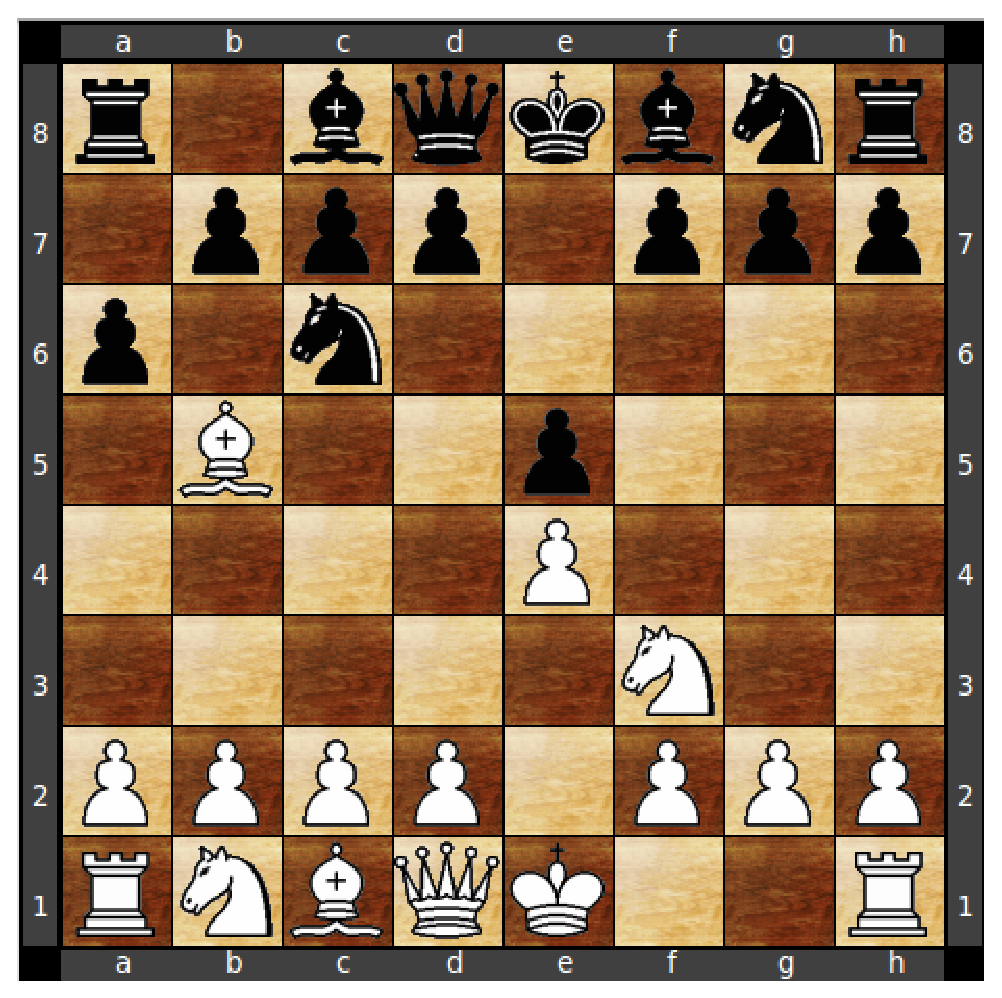
\includegraphics[width=8cm, height=8cm]{diagram1.ps}
\end{center}

V pozici na~diagramu je na~tahu bílý, jedná se o~známou pozici ze zahájení jménem španělská hra (1. e4 e5 2. Jf3 Jc6 3. Sb5), kde se černý brání obvyklým tahem 3. ...a6. Napadl tedy bílému střelce a ten musí hrozbu nějak pokrýt. Běžné tahy jsou nyní 4. Sa4 a Sxc6, hrát by se dalo i Sc4 a snad ještě velmi defenzivní Se2, všechny ostatní tahy jsou již vyloženě špatné. Z této pozice dáme programu za úkol provést propočet do~hloubky dvou půltahů. Vygeneruje tahy a zkouší jeden po druhém zahrát. Generátor tahů je lehce modifikovaný tak, aby vracel braní před ostatními tahy. Program tedy nejprve propočítá 4. Sxc6, projde všechny odpovědi černého a zjistí, že po nejlepším 4. ...dxc6 je pozice přibližně vyrovnaná. Bílý sice ztratil výhodu dvojice střelců, ale zase černému znehodnotil pěšcovou strukturu. Ohodnocení prvního tahu zatím proběhlo tak, jako v~algoritmu {\it minimax}. Rozdíl nastane až u druhého tahu bílého 4. Sxa6. Jedná se o~zjevnou chybu, kterou bílý odevzdává střelce za pouhého pěšce, ale {\it minimax} by musel projít všechny odpovědi, aby si to uvědomil. Tedy poctivě počítat a ohodnocovat nejen 4. ...bxa6 a Vxa6, ale i zcela nesmyslné tahy jako 4. ...Jh6 nebo g5. Modifikovanému algoritmu stačí jediná: 4. ...Vxa6 nebo bxa6. Navíc generátor tahů, který preferuje braní, vrátí jeden z~uvedených tahů hned jako první. Jak program pozná, že může propočet odpovědí na~4. Sxa6 přerušit a prohlásit tah za neperspektivní? Z propočtu 4. Sxc6 si zapamatoval hodnotu nejlepší odpovědi 4. ...dxc6, tedy zhruba 0 tj. vyrovnanou pozici. Při propočtu dalších tahů (4. Sxa6) uvedenou hodnotu použijeme jako práh. Pokud jej jakákoli odpověď (4. ...bxa6 nebo Vxa6) přesáhne, propočet tahu (4. Sxa6) ukončíme, neboť již víme, že je špatný. Jinými slovy: pokud víme, že tah je špatný (= horší než nějaký jiný - zde 4. Sxc6), nemá smysl dále zkoumat, jestli není náhodou ještě o~něco horší, než jsme zatím zjistili.
Pokud počítáme do~hloubky 3 a více, dojde při~prořezávání na~oba hráče a jsou zde proto meze pro obě strany. Dolní se říká {\it alfa}, horní {\it beta}, odtud také název algoritmu alfabeta metoda (nebo {\it alfabeta ořezávání}). Pokud během propočtu narazíme na~variantu, která je horší než {\it alfa}, můžeme ji zahodit. Vyjde-li nám varianta lepší než beta, může se jí zase vyhnout soupeř a zahrát tah, který je lepší pro něj. Časová složitost {\it alfabety} silně závisí na~pořadí tahů, což ovlivňuje, jak rychle se nám podaří sevřít meze {\it alfa} a {\it beta}. Časová složitost optimální {\it alfabety} je \begin{math}v^{h/2}\end{math}, můžeme se s~ní tedy za stejný čas dostat dvakrát hlouběji než s~{\it minimaxem}. Je tudíž žádoucí, aby nejnadějnější varianty počítal algoritmus jako první. Existuje několik heuristik, jak odhadnout už v~generátoru tahů, které varianty by mohly být nejlepší:
\begin{itemize}
	\item {\bf Sežer, co můžeš:} Způsobí-li tah změnu materiálu, posuneme ho na~více dopředu. Preferovat můžeme rovněž braní nižší figurou.
	\item {\bf Historická heuristika:} Je založena na~myšlence, že pokud byl tah dobrý v~jedné variantě, nejspíš bude dobrý i v~jiné. Tři typy této metody mohou být:
	\item {\bf Globální tabulka tahů:} Program si musí nějak pamatovat tahy. Informace, odkud a kam se táhne, případně typ nové figury po proměně pěšce, se při~troše snahy vejde do~16 bitů. Vytvoříme si tedy pole velikosti 216, pro každý možný tah jeden byte. Na počátku propočtu obsahuje pole samé nuly. Když se nějaký tah ukáže jako dobrý (větší než aktuální hodnota {\it alfa}), zvětším hodnotu jeho políčka v~poli. Když potom po vygenerování třídíme tahy, uvažujeme ještě také hodnotu této heuristiky. Jak přesně se mají zvětšovat hodnoty v~tabulce, je složitá otázka. Je zřejmé, že dobré tahy z~pozic vzdálenějších od kořene mají menší význam než dobré tahy z~pozic blízkých kořeni. Je to tím, že průměrná pozice z~propočtu je bližší kořeni než nějakému listu ze vzdálené větve.
	\item {\bf Nejlepší tahy pro danou hloubku:} Pro každou hloubku zanoření v~propočtu si zapamatujeme poslední dva zlepšující tahy. Tyto tahy dostanou při~propočtu v~tomto zanoření speciální bonus. Oproti globální tabulce má metoda tu výhodu, že se více týká aktuální pozice a příslušné hloubky, chová se tedy lokálně. Tím pádem většinou preferuje zlepšující tahy z~blízkých uzlů a u nich je opravdu dost velká pravděpodobnost, že budou dobré i v~počítané pozici. Nevýhodou je, že ohodnocuje jen relativně málo tahů (přesně 2).
	\item {\bf Hlavní varianta:} Program si uchovává v~tabulce dosavadní hlavní variantu, tedy větev výpočtu při~optimální hře (optimální ve~smyslu ohodnocení listů) obou hráčů. Tah, který přísluší k hlavní variantě, bude zřejmě dobrý i v~celé řadě jiných variant, a proto získává bonus. Varianty se ukládají do~matice, využívá se ale jen horní trojúhelník. V jednom políčku matice je jeden tah. Jsme-li při~propočtu v~nějakém uzlu, počítáme v~tomto okamžiku vlastně hodnotu všech pozic na~cestě z~kořene do~našeho uzlu. V i-tém řádku (od diagonály dál) si uchováváme nejlepší dosavadní variantu z~i-té pozice na~cestě od kořene. Dejme tomu, že v~hloubce {\it i} došlo k nalezení zlepšujícího tahu. V řádku {\it i} máme původní nejlepší variantu (od naší pozice dál) a v~řádku {\it i+1} je zlepšující varianta. Za této situace musíme zkopírovat i+1-ní řádek na~pozici i-tého (z něj zůstane jen první tah na~diagonále).
\end{itemize}
Nevýhodou {\it alfabety} je její pevná hloubka. Jsme-li v~zahájení nebo střední hře, bude tahů k ohodnocení velmi mnoho. Hloubka výpočtu v~této části hry by tedy neměla být příliš vysoká, jinak se k výsledku nedopočítáme v~rozumném čase. Naopak v~koncovce, kdy je pouze pár přípustných tahů, lze hloubku propočtu zvýšit.
Tento problém řeší {\it kaskádová metoda}. Jedná se vlastně o~{\it alfabeta metodu}, která postupně počítá do~hloubky 1,2,3,...,n. Na první pohled se může zdát zbytečné počítat pokaždé znovu, nicméně {\it kaskádová metoda} má několik výhod:

\subsubsection{Zpomalení je malé}

Protože je složitost {\it alfabety} exponenciální, zpomalí {\it kaskádová metoda} program cca jeden a půl krát. Dejme tomu, že průměrný větvící faktor šachu je 38, při~dobrém {\it alfabeta ořezávání} se dostaneme na~větvící faktor zhruba odmocnina z~38, přiližně 7. \begin{math}!7^{n-1}\end{math}je zhruba o~řád menší než \begin{math}7^n\end{math}.

\subsubsection{Lepší časová kontrola}

V praxi obvykle nezní zadání \uv{dej mi nejlepší tah do~hloubky 5}, ale \uv{dej mi nejlepší tah, máš na~to 5 sekund}. Potom je velmi obtížné stanovit hloubku propočtu, kterou dosáhneme v~daném čase. U {\it kaskádové metody} prostě provádíme iterace tak dlouho, dokud máme čas. To nám právě umožní v~koncovce (případně kdykoliv, když je množina možných tahů dostatečně malá) počítat do~větší hloubky.

\subsubsection{Třídění tahů}

{\it Kaskádová metoda} poskytuje lepší možnosti třídění tahů. Propočet do~hloubky {\it 1} začneme s~tahy setříděnými podle jednoduchých heuristik v~generátoru tahů. Nejlepší tah poté přemístíme na~začátek, pokračujeme propočtem do~hloubky 2, nejlepší taj z~hloubky 2 opět přemístíme na~začátek a tak dále. Tím se nám podaří velmi rychle sevřít interval {\it alfa} a {\it beta} okolo nejnadějnějších tahů, což {\it kaskádovou metodu} ještě dále zrychlí. Případů, kdy zahájíme propočet několika špatnými tahy, bude velmi málo - obvykle se jedná o~pozice s~možností složité oběti nebo komplikovaného tahu.

\subsubsection{Metoda okénka}

{\it Alfabeta metoda} svírá interval {\it alfa} a {\it beta} velmi defenzivně tak, aby se vždy dopočítala ke správnému výsledku. Celý výpočet můžeme zrychlit tím, že meze {\it alfa} a {\it beta} ještě více sevřeme - vytvoříme interval {\it alfa2} a {\it beta2}, který bude podmnožinou původního {\it alfa} a {\it beta}. Pokud jsme měli pravdu, ušetřili jsme na~výpočtu nějaký čas, pokud ne, interval prostě přeteče a v~následující iteraci {\it kaskádové metody} se počítá interval s~již opravenými mezemi.

\subsubsection{Prohlubování}

Herní algoritmus počítá do~nějaké hloubky, na~jejímž konci ohodnotí pozici statickou ohodnocovací funkcí. Tento postup dobře funguje v~běžných pozicích, ale v~taktických (jako je výměna těžkých figur, pozice tah před matem, kdy vítězná strana obětovala materiál, atp.) selhává. Přitom by zde stačila o~něco málo větší hloubka propočtu a program by hrozby včas viděl. Celkovou hloubku propočtu nemůžeme příliš zvyšovat - program by se nedopočítal. Řešením je tedy prohloubení těch variant, které jsou obzvláště zajímavé.

\subsubsection{Dopočet do~tiché pozice}

Dopočet do~tiché pozice patří v~šachu k nejjednodušším a zároveň nejdůležitějším vylepšením {\it alfabeta metody}. Na úroveň hry programu má zcela zásadní vliv. Spočívá v~tom, že pokud se v~propočtu dostaneme do~listu, neodhadujeme hodnotu pozice statickou ohodnocovací funkcí, ale jakousi modifikací {\it alfabety}, která se liší tím, že bere v~úvahu pouze braní a proměny pěšce. Vzhledem k tomu, že hráči odepíráme všechny ostatní tahy (tzv. tiché tahy), musíme mu umožnit nehrát, jinak bychom jej nutili i do~nevýhodných braní. Funkce tedy vrací maximum z~hodnoty pozice odhadnuté statickou ohodnocovací funkcí a rekurzivního dopočtu braní. Právě dopočet do~tiché pozice řeší případy nedopočítaných výměn. Dopočet samozřejmě hodně zdržuje a sníží základní hloubku propočtu, ale pozitivní efekt je i tak obrovský. Dopočet do~tiché pozice má navíc kladný vliv i na~stabilitu výpočtu - již se nám nestane příliš často, že by zvýšení základní hloubky propočtu mělo nějaký zásadní vliv na~hodnotu varianty.

\subsubsection{Prohlubování taktických variant}

Dopočet do~tiché pozice je účinný, ale neřeší vše. Ve~zvlášť nadějných variantách bývá dobré hloubku propočtu o~jedničku zvýšit a nemusí se při~tom nutně jednat o~braní nebo proměny pěšce. K prohloubení také nemusí dojít jen v~listu. Kdy přesně má smysl prohlubovat, je složitá otázka. Za typické kandidáty na~prohloubení můžeme označit tahy:
\begin{itemize}
	\item Kdy je sebraná figura, která v~minulém tahu sama brala (může se jednat o~dokončení výměny)
	\item Pokrytí šachu představením (může být jen oddálením matu skrývajícího se za horizontem propočtu)
	\item Jakékoliv varianty s~vynucenými tahy
	\item Vidle pěšcem i jezdcem a podobné taktické údery
	\item Varianty s~tzv. {\it Fisherovým střelcem}
	\item Taktické hrozby králi
\end{itemize}
Při prohlubování je potřeba postupovat velmi obezřetně, neboť prohloubení jedné varianty zkrátí výpočetní čas ostatních variant.

\subsubsection{Haš tabulky}

Až do~tohoto okamžiku jsme se snažili zrychlit výpočet pomocí ořezávání a svírali jsme interval {\it alfa} a {\it beta}, jak to jen bylo možné, abychom odřízli co nejvyšší počet variant, které nemá smysl počítat. Existuje však ještě jeden druh variant, které rovněž nemusíme počítat. Jde o~dvojice variant, které se od sebe liší pouhým prohozením tahů. Pokud program počítá do~hloubky 5 půltahů ze základního postavení, nevynechá ani variantu bílý pěšec na~e4, černý pěšec na~c5 v~prvním tahu, bílý jezdec na~f3 v~druhém tahu a z~této pozice počítá ještě do~zbývající hloubky 2 půltahy. Ke stejnému výsledku se však dostane i z~pozice, kdy v~prvním tahu přijde bílý jezdec na~f3 a černý pěšec na~c5 a ve~druhém tahu bílý pěšec na~e4. Následující dva půltahy se budou počítat znovu. Je přitom zřejmé, že vzniklou pozici stačí zkoumat jen jednou.
V zahájení a střední hře s~velkým počtem figur a malou hloubkou propočtu dochází k těmto duplicitám ještě poměrně zřídka. Mnohem horší je situace v~koncovce s~malým počtem figur. Typickým příkladem je koncovka dvou králů, v~níž mají obě strany už jen několik zablokovaných pěšců. Král se obvykle snaží vytlačit soupeřova monarchu (obvykle i s~využitím nevýhody tahu), pobrat soupeřovy pěšce a prosadit ty své do~dámy. Obě strany přitom mají na~výběr jen několik málo přípustných tahů, a tak hloubka propočtu roste oproti střední hře i dvojnásobně. Při podobných hlubokých propočtech dochází k opakovanému vyhodnocování jedné varianty, vzniklé jen přehozením tahů, zcela běžně. Právě v~podobných typech pozic přitom může mít počítač s~lidským soupeřem problémy. Jednoduchý charakter pozice totiž umožní lépe oprostit plán výhry nebo obrany od detailního propočtu (případně lidský propočet degeneruje na~jedinou, ale zato dlouhou variantu bez větvení) a umožní vidět mnohem dál i člověku.

Řešením je mít haš tabulku s~výsledky jednotlivých výpočtů, do~které se podíváme, a pokud zde výsledek propočtu z~naší pozice najdeme, okamžitě ho vrátíme. Je nutné dát pozor na~několik věcí:
\begin{itemize}
	\item Ukládat je třeba i hloubku propočtu, neboť nelze nahradit propočet výsledkem předchozího propočtu do~menší hloubky.
	\item {\it Alfabeta} nedává jen mezivýsledky typu \uv{pozice má cenu = 3}, ale i \uv{pozice má cenu $\le$ 3} nebo \uv{pozice má cenu $\ge$ 3}. Tyto mezivýsledky je rovněž nutné ukládat.
	\item Musíme pracovat velmi rychle s~velkým množstvím dat.
	\item Program by neměl číst z~disku - struktura se musí za každou cenu vejít do~paměti.
	\item Je lepší, když struktura zapomíná než aby swapovala
	\item Pozice obsahuje 64 polí a stavovou informaci o~tahu, právu na~rošády a braní mimochodem, ale jeden záznam ve~struktuře by měl mít Jen několik bytů, proto volíme haš tabulku.
\end{itemize}

V této haš tabulce nemusíme řešit kolize - nová nebo cennější hodnota prostě přepíše starou. Je to rychlejší a jednodušší než na~jednotlivých prvcích vytvářet spojové seznamy a zabývat se alokováním a uvolňováním paměti.

\subsubsection{Databáze zahájení a koncovek}

Každá šachová partie začíná vždy stejnou pozicí. Je celkem pochopitelné, že šachisté velmi pečlivě studují jednotlivé varianty vzniklé ze základního postavení již v~klidu doma s~počítačem nebo v~klubu během tréninku a ne až v~omezeném čase během partie. O konkrétních zahájeních byly napsány stovky knih, věnovali se jim ti nejlepší šachisté teoretici. Během zahájení běžně vznikají velmi komplikované pozice, ve~kterých se nevyznají ani velmistři, a malá nenápadná a těžko odhalitelná chyba může vést k rychlé prohře nebo alespoň k výhodě soupeře. Rozmotat přímo za šachovnicí několik delších a trochu rozvětvených vynucených variant (které během desítek let vymysleli šachoví teoretici) bývá bez předchozí přípravy nad síly i těch nejlepších hráčů a dnešních programů, ale naučit se řešení nazpaměť a pochopit ho dokáže při~troše snahy i průměrný klubový šachista nebo třeba náš program.
Program naučíme zahájení tak, že někam uložíme pozice běžné v~zahájení a/nebo jejich haš funkce a k nim sadu tahů, které od programu v~uvedené pozici očekáváme. Každému tahu zároveň přiřadíme pravděpodobnost jeho zahrání. Například pro základní postavení může seznam vypadat takto:
\begin{itemize}
	\item 30\% 1. e4
	\item 30\% 1. d4
	\item 15\% 1. c4
	\item 13\% 1. Jf3
	\item 5\% 1. f4
	\item 2\% 1. b3
	\item 1\% 1. b4
	\item 1\% 1. g3
	\item 1\% 1. e3
	\item 1\% 1. d3
	\item 1\% 1. Jc3
\end{itemize}

Největší pravděpodobnost budou mít dobré a obvykle hrané tahy, méně běžným a nepříliš ambiciózním tahům, které však pozici bílého nijak neohrožují, dáme jen malou pravděpodobnost (hodí se občas k vyprovokování lidského soupeře) a tahy vyloženě špatné jako například 1.f3? nebo 1.h3?, nebudeme uvádět vůbec, program je tedy nebude hrát.
Podobný seznam pravděpodobností ohodnocených tahů budeme mít pro každou naučenou pozici uložený v~nějaké datové struktuře postavené nad hašovací funkcí pozice. Tahů z~pozic je proměnlivé množství. Typická vyhledávací datová struktura proto nebude obsahovat přímo tahy. Místo nich v~ní budou indexy do~pole tahů zakončené nulou. Ukážeme si to na~příkladu se setříděným polem a hašovací funkcí, která není na~naší množině uložených pozic prostá. Obsahovat bude jen 3 pozice: základní postavení (haš = 368) se třemi tahy 1. e4 (40\%), 1. d4 (40\%) a 1. c4 (20\%), pozici po 1. e4 (haš = 129) se dvěma tahy 1. ...c5 (50\%) a 1. ... e5 (50\%) a nakonec pozici po 1. e4 e5

\vskip 0.5cm
\noindent
\begin{tabular}{|l|l|l|}
\hline
haš 129, index 0 & haš 368, index 3 & haš 368, index 5 \\
\hline
pozice po 1. e4 & pozice po 1. e4 e5 & základní postavení \\
\hline
\end{tabular}
\vskip 0.5cm

Takto by vypadala vyhledávací struktura. Pozice bychom si pamatovali nejspíš fyzicky odděleně, například na~stejném indexu v~jiném poli, zde je proto máme v~druhém řádku. Dejme tomu, že hledáme tah ze základního postavení. Spočítáme si hašovací funkci 368. Nějakým algoritmem pro vyhledávání v~setříděném poli s~rovnoměrným rozdělením dat (logaritmicky půlením nebo ještě lépe dělením podle hodnoty haš funkcí) najdeme políčko se správnou hodnotou haš funkce, dejme tomu, že máme smůlu, a bude to prostřední políčko. Zjistíme, že pozice není naše, neboť došlo ke kolizi haš funkcí. Podíváme se {\it while} cyklem doleva, a vidíme tam už jinou hodnotu haš funkce. Podíváme se tedy doprava na~poslední políčko. Zde odpovídá haš funkce a také pozice je správně, budeme tedy hledat tahy na~indexu 5 v~poli tahů. Tabulka tahů pak může vypadat zhruba takto:

\vskip 0.5cm
\noindent
\begin{tabular}{|c|c|c|c|c|c|c|c|c|}
\hline
0 & 1 & 2 & 3 & 4 & 5 & 6 & 7 & 8 \\
\hline
c5 (50\%) & e5 (50\%) & 0 & Jf3 (100\%) & 0 & e4 (40\%) & d4 (40\%) & c4 (20\%) & 0 \\
\hline
\end{tabular}
\vskip 0.5cm


V poli od pozice 5 až k následující nule jsou tahy e4, d4 a c4, vygenerujeme tedy náhodné číslo z~rozsahu 0 až 100, padne třeba 50 a program zahraje 1. d4.

S ubývajícím počtem figur a blížícím se koncem partie se pozice postupně zjednodušuje. Při propočtu ubývá možných variant, spousta z~nich vede do~stejné pozice, jiné zase brzy končí matem nebo remízou. Program by měl tudíž v~jisté chvíli začít počítat dokonale. Pokud však zkusíme standardnímu prohledávacímu algoritmu předložit třeba nějakou pozici z~koncovky střelce a jezdce proti samotnému králi, kvalitní program koncovku sice zvládne - zatlačí soupeřova krále do~rohu barvy střelce a tam mu nasadí mat, ale rozhodně nenajde ten nejrychlejší postup a maty třeba 20. tahem zdálky prostě neuvidí. V opravdu těžkých koncovkách typu dáma proti dvěma lehkým figurám pak běžný kvalitní myslící algoritmus již bude chybovat a některé vyhrané pozice vyhrát nedokáže. V omezeném čase není možné ani v~poměrně jednoduché koncovce projít celý graf hry z~kořene k listům, díky kolizím v~hašovací funkci navíc budeme řadu variant počítat opakovaně, takže s~dokonalou hrou nemůžeme počítat ani v~elementární koncovce dámy proti samotnému králi.
Naštěstí je to s~pozicemi z~koncovek podobné, jako s~těmi ze zahájení. Dají se naučit. Všech možných pozic několikafigurové koncovky je sice z~lidského pohledu mnoho, ale počítač má posunutá měřítka. Jednoduchý horní odhad pro počet pozic n-figurové koncovky je \begin{math}2 * 64^n\end{math}, neboť každá figurka může být na~jednom ze 64 polí a možnosti se násobí. Úvodní dvojka je tam kvůli právu tahu, buď hraje bílý nebo černý. Náš odhad bychom mohli i zpřesnit na~2 * 64 * 63 * 62 * ... * (64 - n + 1), protože dvě figurky nemohou být na~stejném políčku, takže první figurka má 64 možností, druhá jen 63 atd. Mohli bychom také vyškrtat nepřípustné pozice, ztotožnit stejné figury atd., ale úvodní vzorec nám zároveň dává návod, jak velmi jednoduše a efektivně každé pozici zkoumané koncovky přidělit číslo od 0 do~\begin{math}2 * 64^{n-1}\end{math} (její místo v~tabulce příslušné koncovky) a naopak ke každému číslu z~uvedeného intervalu přiřadit pozici.
Stanovíme si pořadí figur naší koncovky podle jejich barvy a materiální hodnoty. Například pro koncovku jezdce a střelce to může být pořadí bílý král, bílý střelec, bílý jezdec, černý král. Očíslujeme políčka šachovnice od 0 do~63, přičemž a1 bude 0, a2 bude 1 atd., h8 bude 63. Máme-li {\it n} jednoznačně seřazených figur, označíme čísla políček, na~nichž se nacházejí, \begin{math}p_0\end{math} až \begin{math}p_{n-1}\end{math}. U koncovek s~opakováním jednoho druhu kamene (například koncovka krále proti dvěma střelcům) budeme jako první uvažovat figuru s~vyšším indexem políčka. Číslo pozice pak bude \begin{math}p_0 + 64 * p_1 + 64^2 * p_2 + ... + 64^{n-1} * p_{n-1} + (\end{math}hraje bílý ? \begin{math}64^n : 0)\end{math}.

\begin{center}
	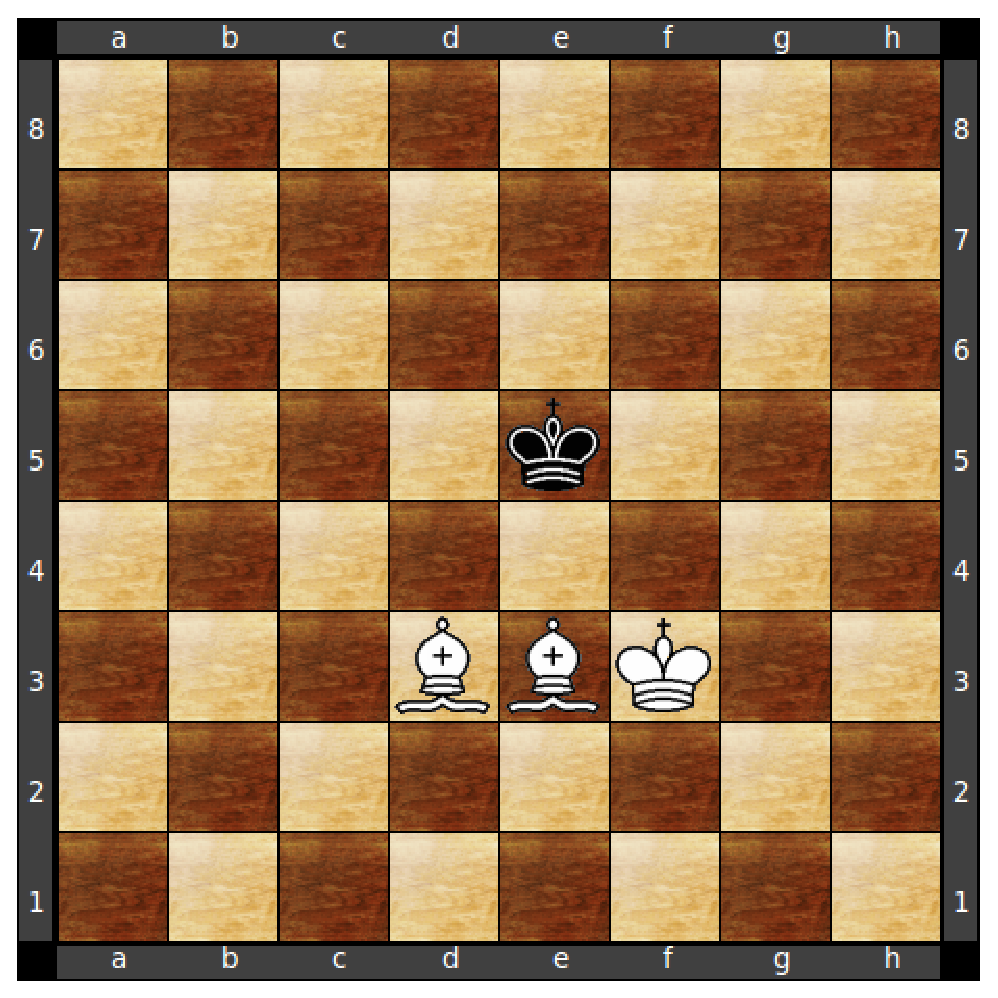
\includegraphics[width=8cm, height=8cm]{diagram2.ps}
\end{center}

Na obrázku je příklad pozice z~koncovky dvou střelců. Pořadí figur bude KSSk, tedy bílý král a oba střelci a nakonec černý král. Na tahu je bílý a na~naší šachovnici hraje nahoru, střelci jsou tedy na~d3 a e3, bílý král na~f3 a černý na~e5. V následující tabulce je výpočet čísla pozice v~rámci dané koncovky. Výsledek je 26 293 525.

\vskip 0.5cm
\noindent
\begin{tabular}{|l|c|c|r|r|}
\hline
	{\bf Figurka} & {\bf Pole} & {\bf Index} & {\bf Hodnota} & {\bf Výsledek} \\
\hline
	Bílý král & f3 & 21 & 21 & 21 \\
\hline
	První bílý střelec & e3 & 20 & \begin{math}20 * 64\end{math} & 1 280 \\
\hline
	Druhý bílý střelec & d3 & 19 & \begin{math}219 * 64^2\end{math}	& 77 824 \\
\hline
	Černý král & e5 & 36 & 36 * \begin{math}264^3\end{math} & 9 437 184 \\
\hline
	\multicolumn{3}{|l|}{Bílý na~tahu} & \begin{math}264^4\end{math} & 16 777 216 \\
\hline
	\multicolumn{4}{|l|}{Suma} & 26 293 525 \\
\hline
\end{tabular}
\vskip 0.5cm

Opačný převod z~čísla na~pozici bude analogický, číslo rozložíme na~cifry v~64-kové soustavě a to budou indexy políček jednotlivých kamenů.

Vlastní algoritmus vygenerování databáze n-figurové koncovky bude vypadat přibližně takto:
\begin{itemize}
	\item Rekurzivně stejným algoritmem vygeneruj databáze koncovek, které z~naší koncovky mohou vzniknout. (Například pro koncovku dámy proti věži vygeneruj nejprve koncovku se samotnou dámou a se samotnou věží.)
	\item Naalokuj místo pro \begin{math}2 * 64^n\end{math} čísel a vyplň je nulami
	\item Projdi přirozená čísla od 0 do~\begin{math}2 * 64^n -1\end{math}, ke každému vygeneruj pozici. Je-li nepřípustná (2 figury na~sobě, šach nehrajícímu), vlož do~pole čísel na~daný index konstantu CHYBA, je-li černý v~matu, vlož 1, je-li bílý v~matu, vlož -1.
	\item Projdi přirozená čísla od 0 do~\begin{math}2 * 64^n -1\end{math}, přeskoč ta, kde je na~daném indexu v~poli jiné číslo než nula. Ke každému číslu vygeneruj pozici. Na náš index do~pole vlož, stručně řečeno, hodnotu propočtu {\it minimaxem} do~hloubky 1 s~ohodnocením pomocí již spočítaných hodnot a nul v~poli. Podrobně řečeno: Dejme tomu, že hraje bílý (pro černého budeme postupovat analogicky). Vygeneruj z~pozice tahy, zahraj je. Pokud zahraným tahem přešla pozice do~jiného druhu koncovky (proměna pěšce, braní), podívej se do~tabulky pro tuto koncovku, kolikátým půltahem bílý dává nebo dostává mat, případně zda je pozice remízová. Pokud zůstal zachován typ koncovky, spočítej si index pozice a podívej se do~pole, zda a jak již máme pozici ohodnocenou. 0 znamená, že zatím nevíme, kladné číslo, že je pozice vyhraná za bílého, záporné, že za černého. Je-li mezi čísly alespoň jedno kladné, vlož do~pole na~náš index to nejmenší z~těch kladných čísel zvětšené o~1. (Například z~0, 0, 0, 5, 3, -2, 0, 0, -2, -4 vyber 3 a do~pole na~náš index dej 3 + 1 = 4. Znamená to, že dáváme mat 2. tahem, neboť jsme o~3 půltahy od 1, což je mat.) Jsou-li všechna čísla záporná, je pozice za bílého prohraná, vyber z~nich tedy to nejmenší (s největší absolutní hodnotou) a do~pole na~náš index ho dej zmenšené o~1. (Například z~-2, -4, -6, -6, -4 vyber -6 a do~pole dej -7. To znamená, že jsme na~tahu a dostáváme mat 3. tahem.) Poslední možností je, že mezi čísly je alespoň jedna 0 a zbytek jsou buď nuly nebo záporná čísla. V tom případě ještě nemůžeme rozhodnout a v~poli necháme nulu.
	\item Pokud jsme zapsali do~pole alespoň jednu nenulu, pokračuj bodem 4.
	\item Ulož pole do~souboru tak, jak je.
\end{itemize}
Máme-li vygenerovanou tabulku, je již velmi jednoduché napsat optimální algoritmus hry. Jedná se o~prostý {\it minimax} do~hloubky 1. Místo běžné ohodnocovací funkce se budeme dívat do~tabulky. 0 znamená, že žádná ze stran nemůže vyhrát, tedy remíza. Kladná čísla jsou pozice vyhrané za bílého, čím dál od jedničky, tím dál od matu. Totéž platí s~černým pro záporná čísla. V remízových pozicích pak můžeme spustit i klasický myslící algoritmus omezený na~tahy, které nevedou k naší prohře. Jde jen o~to, aby v~remízových pozicích, kde ovšem o~remízu bojuje soupeř, program nerezignoval na~teoreticky marnou, ale prakticky proti reálnému soupeři často nadějnou snahu o~výhru a nezahrál prostě jakýkoli neprohrávající tah. Například v~těžké (pro 2 jezdce), ale remízové koncovce dámy proti dvěma jezdcům by program asi neměl nastavit dámu. To sice objektivně není chyba, neboť i koncovka krále a dvou jezdců proti samotnému králi je remízová, ale subjektivně to jistě chyba je a uživatel by to nejspíš programu neodpustil.

Bohužel tento algoritmus není na~současných počítačích dostatečně rychlý - na~počkání získáme jen třífigurové koncovky, přes noc pak čtyřfigurové. Jednou z~nejjednodušších a zároveň velmi účinných metod, jak výpočet zrychlit a zmenšit i objem vygenerovaných dat, je využití nejrůznějších symetrií. 50\% ušetříme, pokud jednotlivé koncovky budeme generovat jen pro jednu stranu tj. nikoliv celkem dvakrát: jednou pro bílého a jednou pro černého. Dále můžeme ušetřit překlápěním šachovnice. Pokud vyloučíme rošády, můžeme pozici ztotožnit s~jejím osově souměrným obrazem, kdy osa vede mezi sloupci {\it d} a {\it e}. Generovat tedy budeme jen pozice, na~nichž je bílý král na~sloupcích {\it a} až {\it d} a jejich dvojčata budeme pomocí osové souměrnosti transformovat. V bezpěšcových koncovkách můžeme podobně překlápět i podle vodorovné osy mezi 4. a 5. řadou a dokonce i podle hlavní diagonály a1 - h8. Bílý král tak bude vždy v~trojúhelníku a1-d1-d4. Místo 64 možných polí tak zbude bílému králi pouze 10 polí, lze tedy očekávat díky osovým souměrnostem zhruba 6,4-násobné zrychlení a úsporu paměti při~generování i při~uložení výsledků.
V tabulce jakékoli koncovky se poměrně často a relativně pravidelně opakují číselné hodnoty. Je zřejmé, že data lze úspěšně komprimovat téměř jakoukoli rozumnou metodou. Vzhledem ke způsobu využití je nutné, aby pro přečtení hodnoty z~komprimované tabulky stačilo dekomprimovat jen nějaké malé okolí a nikoli celou tabulku.

\subsection{Reprezentace pozice}

Nejjednoduší reprezentace šachovnice je dvourozměrné pole 8x8. To můžeme v~případě potřeby rozvinout na~jednorozměrné pole o~64 prvcích. Výhodou tohoto přístupu je snadnější čitelnost programu, nevýhodou je nutnost ošetřit možné přetečení pole. (Např. tah jezdce z~okraje šachovnice mimo její okraj. Toto se dá řešit polem 10x12, potažmo jednorozměrným polem o~120 prvcích, což je vlastně klasická šachovnice 8x8 s~mantinely.

Nejjednodušší reprezentace šachových figur je celým číslem - kladným pro bílé, záporným pro černé. Prázdné pole je pak neutrální a má hodnotu 0, mantinely (jsou-li přítomny) mají nějakou konstantní hodnotu, která se neuvažuje pro výpočet.

Další možnou reprezentací šachovnice může být bitové pole. Nějaký jev na~šachovnici je pak reprezentován 64-bitovým číslem. Například výskyt bílých věží v~základním postavení je reprezentován číslem 129 (00000000 00000000 00000000 00000000 00000000 00000000 00000000 10000001) Když budeme mít pro každý typ kamene jednu proměnnou, 12 proměnných může reprezentovat celou šachovnici. Výhodou tohoto přístupu je velmi efektivní zpracování zejména na~64-bitové architektuře, kde je každá operace jedna velmi jednoduchá instrukce. Nevýhodou je, že zejména pro začínající programátory může být tento přístup velmi matoucí a nečitelný.

\subsection{Reprezentace pole tahů}

Protože tahů bude v~průběhu výpočtu generováno velmi mnoho, měl by být typ reprezentující tah velmi malý. Každopádně musí obsahovat minimálně položky odkud a kam. V případě reprezentace šachovnice dvourozměrným polem, budou položky odkud a kam reprezentovány dvouprvkovým polem - na~indexu 0 bude sloupec, na~indexu 1 řádek. V případě, že je šachovnice reprezentována jednorozměrným polem, položky odkud a kam jsou reprezentovány pouze celým číslem.

K uložení množiny tahů se běžně používá globální zásobník tahů, který může vypadat zhruba takto:
\begin{verbatim}
Move moves[MANY]
int borders[DEPTH]
int index_in_stack
\end{verbatim}

Tahy jsou uloženy v~jediném globálním jednorozměrném poli, přičemž tahy z~aktuálně propočítávané pozice mají index {\tt borders[index\_in\_stack]} až {\tt borders[index\_in\_stack+1]-1}. Konstanta {\tt DEPTH} je nejvyšší možná hloubka zanoření rekurze. Na dnešních počítačích by mělo stačit 32. Velikost konstanty {\tt MANY} pak půjde shora odhadnout jako součin maximálního počtu tahů z~pozice * {\tt DEPTH}. Program při~tomto postupu sice může trochu plýtvat pamětí, ale achillovou patou šachových programů obvykle nebývá nedostatek paměti, nýbrž nedostatek času na~dostatečně hluboký výpočet. Toto řešení ušetří cenné mikrosekundy, které by stálo dynamické přealokovávání pole v~cyklu.

\subsection{Ohodnocovací funkce}

Šachový program provádí propočet do~určité hloubky, na~jehož konci zavolá ohodnocovací funkci, která vrátí cenu dané pozice. Nejjednodušší a nejdůležitější je samozřejmě sečíst materiál. Cena jednotlivých figur se v~různých programech liší. Pokud má pěšec cenu 1, bude cena jezdce a střelce přibližně 3, věže 5 a dámy 9. Někdy bývá hodnota střelce nepatrně vyšší než hodnota jezdce a podobně. Šachový program s~ohodnocovací funkcí degenerovanou na~prostý součet materiálu se pochopitelně bude chovat divně. Cesta i od velmi zjevné poziční chyby k matu je velmi dlouhá a přesahuje hloubku propočtu dnešních programů, takže prostý součet materiálu nestačí. Proto se přidává poziční složka.
Poziční složka bývá obyčejně velmi malá, jen zřídka v~reálných partiích přesáhne v~absolutní hodnotě cenu pěšce. Řada pozičních faktorů se dá ocenit statickou tabulkou pro jednotlivá políčka. Například poziční bonus pro figury blíže ke středu šachovnice (a tím i větším manévrovacím prostorem) bude vyšší než pro figury u kraje nebo v~rohu šachovnice. Takovéto řešení poziční složky jistě nebude dokonalé, zato bude velmi rychlé. Poziční tabulku můžeme pro jednotlivé figury lehce upravit.

Pro pěšce existuje celá řada heuristik. Můžeme pozičně více ocenit pěšce, kteří jsou dále od výchozího postavení - to pěšce přiměje utíkat směrem k dámě. V základním postavení pak můžeme ocenit vyšším bonusem pěšce, kteří vykročí na~středu. Dále můžeme ocenit, je-li pěšec volný (žádná figura mu nebrání v~běhu do~dámy), či je-li krytý jiným pěšcem. Rovněž může dostat postih, je-li opožděný.

Jezdec stojí dobře v~centru, v~rohu se mu obvykle nedaří. Rovněž můžeme ocenit jezdce šikovně krytého pěšcem.

Pro střelce sice není poziční ohodnocení tak podstatné, přesto se o~to můžeme pokusit. Dobře umístěný střelec by měl dostat bonus za soupeřovy pěšce na~stejné barvě pole, které může napadat, a naopak postih za pěšce, které napadat nemůže. Tím nám vyjde, že dva střelci budou mít spolu nepatrně vyšší hodnotu, než je prostý součet jejich hodnot.

U věže nemá statická ohodnocovací tabulka smysl. Věž patří na~volný sloupec, má tlačit na~opožděné nebo nekryté pěšce a obě věže by se měly navzájem krýt.

U dámy je potřeba snad jen zabránit předčasnému vývinu - soupeř pak prostě napadá dámu s~tempy běžných vývinových tahů lehčích figur.

U krále je v~zahájení a střední hře důležitá především bezpečnost. Jde jednak o~umístění, zachované právo rošády, pěšcový kryt krále a napadnutelnost polí v~okolí. V koncovce se úloha krále radikálně mění a stává se z~něj aktivně bojující figura, která musí opustit úkryt a bojovat o~střed. V matové koncovce se pak král silnější strany snaží přiblížit soupeřovu  králi.

Ohodnocovací funkce napsaná pomocí statických tabulek je velmi rychlá, ale má jednu vážnou slabinu. Tabulky jsou napsány obecně, mohou tedy být dobré pro běžnou pozici, ale stačí několik netypických tahů a správné ohodnocení políček například pro jezdce může být úplně jiné. Řešením je místo samotného pole oceňovat pohyblivost figur, napadnutelná pole a tak podobně. To vše je ovšem za cenu vyšší časové náročnosti.

\section{Popis implementace}

Program je rozdělen na~4 moduly:
\begin{itemize}
	\item {\tt main.c} s~hlavičkovým souborem {\tt zcuchess.h} obsahuje hlavní funkci a pomocné funkce pro správu paměti
	\item {\tt io.c} s~hlavičkovým souborem {\tt io.h} funkce pro vstupní a výstupní operace
	\item {\tt chess.c} s~hlavičkovým souborem { \\t chess.h} základní rutiny umožňující šachovou hru
	\item {\tt ai.c} s~hlavičkovým souborem {\tt ai.h} obsahuje umělou \uv{inteligenci}
	\item {\tt types.h} - hlavičkový soubor s typy
\end{itemize}

\subsection{Globální datové struktury}
\begin{itemize}
	\item {\tt int chessboard[8][8]} reprezentace šachovnice potažmo pozice
	\item {\tt bool castlings[4]} pole s~příznaky rošád, které ještě můžeme provést (malá bílá, velká bílá, malá černá, velká černá)
	\item {\tt int en\_passant[2]} udržuje aktuální pozici pěšce, kterého můžeme sebrat mimochodem. Na indexu 0 je sloupec, na~indexu 1 je řádek
	\item {\tt bool human\_move} příznak, zda-li je na~tahu člověk
	\item {\tt int position\_bonus[8][8]} tabulka s~pozičními bonusy pro statickou ohodnocovací funkci
\end{itemize}

\subsection{Reprezentace šachovnice, pozice a hodnot figur}
Pro názornost byla za reprezentaci šachovnice, potažmo pozic, zvolena matice 8x8. Bílé figury jsou reprezentovány celým kladným číslem následovně:
\begin{itemize}
	\item 1 Pěšec (konstanta {\tt PAWN}), hodnota 100 (konstanta {\tt PAWN\_VALUE})
	\item 2 Věž (konstanta {\tt ROOK}), hodnota 400 (konstanta {\tt ROOK\_VALUE})
	\item 3 Jezdec (konstanta {\tt KNIGHT}), hodnota 300 (konstanta {\tt KNIGHT\_VALUE})
	\item 4 Střelec (konstanta {\tt BISHOP}), hodnota 350 (konstanta {\tt BISHOP\_VALUE})
	\item 5 Dáma (konstanta {\tt QUEEN}), hodnota 750 (konstanta {\tt QUEEN\_VALUE})
	\item 6 Král (konstanta {\tt KING})
\end{itemize}
Černé figury jsou reprezentovány stejně, akorát s~opačným znaménkem. Číslo 0 (konstanta EMPTY) pak reprezentuje prázdné pole.

\subsection{Reprezentace tahu a množiny tahů}

Tah je reprezentován datovou strukturou Move:
\begin{verbatim}
typedef struct {
  int from[2];	//na indexu 0 je sloupec, odkud se táhne, na indexu 1 
								//je řádek odkud se táhne
  int to[2];		//na indexu 0 je sloupec, kam se táhne, na indexu 1 je řádek, 
								//kam se táhne
  bool status;	//příznak, je-li tah validní
} Move;
\end{verbatim}

V programu jsou pro indexy polí {\it from} a {\it to} připraveny konstanty {\it COL} (sloupec, index 0) a {\it ROW} (řádek, index 1). V celém programu se pak tyto souřadnice používají konzistentně, tzn. vždy je sloupec první a řádek druhý.

Množina tahů se ukládá do~struktury Moves:
\begin{verbatim}
typedef struct {
  int count;	//Počet tahů v množině
  Move *move;	//Pole tahů
} Moves;
\end{verbatim}

\subsection{Statická ohodnocovací funkce}
Provádí prostý součet hodnoty materiálu a připočítává poziční bonus. Poziční bonus je reprezentován maticí 8x8 typu int a je pro všechny figury stejný. Vychází z~myšlenky, že každá figura je užitečnější blíže ke středu šachovnice.

\subsection{Myslící algoritmus}
Jako myslící algoritmus byl postupně použit {\it minimax}, {\it alfabeta} a nakonec velmi prostá implementace {\it kaskádové metody}. Všechny tyto algoritmy jsou popsány v~části o~analýze.

\section{Uživatelská příručka}

\subsection{Instalace}

Pokud jste uživateli Linuxu:
\begin{itemize}
	\item V kořenovém adresáři projektu napište do~konzole příkaz {\it make}.
\end{itemize}
Pokud jste uživateli Windows 7:
\begin{itemize}
	\item Stáhněte a nainstalujte libovolný C překladač (např. MinGW).
	\item Klikněte na~tlačítko {\bf Start} a vyberte položku {\bf Tento počítač}.
	\item Klikněte pravým tlačítkem myši do~okna, které se vám zobrazilo, a z~menu vyberte {\bf Vlastnosti}.
	\item V následujícím okně vyberte vpravo položku {\bf Upřesnit nastavení systému}, otevře se další dialogové okno.
	\item V tom klikněte na~tlačítko {\bf Proměnné prostředí...} vpravo dole. Zobrazí se okno, v~němž je možné nastavit proměnné systému.
	\item Najděte proměnnou {\it PATH} a klikněte na{\bf Upravit}. Na konec této proměnné napište za středník cestu k adresáři obsahujícímu soubor gcc.exe (Tedy např.: ;C:$\backslash$MinGW$\backslash$bin$\backslash$)
	\item Pokud proměnná {\it PATH} neexistuje, vytvořte ji.
	\item Pozavírejte všechna okna.
	\item Znovu klikněte na~tlačítko {\bf Start}, vyberte {\bf Příslušenství} a {\bf Příkazový řádek}.
	\item V příkazovém řádku přejděte do~složky projektu a napište {\tt mingw32-make}.
\end{itemize}

\subsection{Ovládání}

Program je konzolový, ovládá se tedy z~klávesnice. Spustíme ho klasicky příkazem ./zcuchess (zcuchess.exe na~platformě Windows). Program při~spuštění vypíše hlavičku, jejíž součástí je i nápověda, a čeká na~zadání prvního tahu. Tah se zapisuje ve~formátu odkud mezera kam, tedy např. {\tt e2 e3}. Poté program chvíli přemýšlí, načež vypíše svůj tah. Automaticky se předpokládá, že člověk hraje za bílého. Nápovědu je možno kdykoliv vypsat vepsáním klíčového slova {\tt help} namísto tahu. Stejně tak je možné program kdykoliv ukončit vepsáním slova {\tt exit} namísto tahu. Pokud nastane mat, program se ukončí sám.

\section{Závěr}
Program hraje šachy dostatečně dobře na~to, aby v~nich porazil svého tvůrce, zadání semestrální práce proto považuji za splněné, i když k dobré hře má program stále ještě velice daleko.

\subsection{Problémy v~průběhu psaní programu}
Při běhu programu docházelo ke značným únikům paměti, které se nakonec podařilo najít a vyřešit za pomoci programu {\it Valgrind}.
Větší problémy nastaly při~pokusech přeložit program na~systému Windows, a to zejména:
\begin{itemize}
	\item Bylo potřeba si opatřit počítač vybavený tímto systémem. Nakonec jsem použil virtuální server s~Windows, který máme k dispozici na~pracovišti.
	\item Nastavení proměnné prostředí {\it PATH}. Zde bych chtěl poděkovat kolegovi Karlu Vlčkovi za trpělivost.
	\item Samotná práce s~příkazovým řádkem ve~Windows.
	\item Po překladu jsem zjistil, že se špatně vypisují znaky s českou interpunkcí, proto jsem program upravil tak, aby používal {\it cestinu}.
	\item Funkce {\tt clock()} nevracela ve~Windows správné výsledky, změnil jsem ji tedy na~funkci {\tt time()}.
\end{itemize}
Na poslední chvíli jsem při~hře svého programu proti programu GNU Chess 4 objevil chybu v~rošádě - program sice kontroloval, zda-li nebylo táhnuto králem či věží a zda-li není král před, po a během rošády v~šachu, ale už nekontroloval, jestli je věž ještě na~svém místě.

\subsection{Možná vylepšení}
Podle profileru tráví program až čtvrtinu času ve~funkci {\tt add\_move} (přidání tahu do~množiny tahů). Toto by se dalo vyřešit globálním zásobníkem tahů. Protože je globální zásobník tahů statický, nebylo by zároveň potřeba řešit úniky paměti.
Dalším vylepšením zlepšujícím hloubku propočtu by bylo nasazení nějakých heuristik do~generátoru tahů a třídění tahů po průběhu {\it kaskádové metody}. V podstatě nasazení jakýchkoli heuristik uvedených u {\it kaskádové metody} v~analýze.
Hru programu by samozřejmě zlepšila také implementace databáze zahájení a koncovek.
Dalším drobným zrychlením by bylo rozvinutí pole 8x8, reprezentujícího šachovnici, na~jednorozměrné pole o~64 prvcích. Vůbec nejzajímavější by bylo použít reprezentaci v~podobě bitové mapy, ale to by si vyžádalo několik měsíců studia.
Z uživatelského hlediska by se jistě hodila možnost dát uživateli na~výběr barvu strany, za kterou chce hrát, či možnost partii uložit do~souboru a opětovně načíst.

Program byl vyvíjen v~integrovaném vývojovém prostředí NetBeans IDE 7.2.1 na~platformě Xubuntu Linux. Mezi další nástroje použité při~vývoji patří Valgrind, verzovací systém GIT a editor VIM.
Postupný vývoj programu a jeho zdrojové kódy si lze prohlédnout na~adrese {\it https://github.com/ClaryAldringen/ZCUChess}.
\end{document}